
\noindent We continue our discussion of systems that exhibit conformal symmetries. These symmetries are contained in the conformal group called $\text{Conf}(\mathbb{R}^{p,q})$, which is the connected component containing the identity of all conformal diffeomorphisms of the pseudo-Riemannian manifold $\mathbb{R}^{p,q}$. \\

\noindent We discussed the infinitesimal conformal transformation, which led to a Lie algebra, the Witt algebra, in $(1+1)$ and $(2,0)$ dimensions. For $d = p+q = 2$, there is a bigger symmetry group (less constrained), yielding more conserved quantiteis, more degrees of freedom of the system. If $d \ne 2$, the symmetry group is too constrained to be that interesting. \\

\noindent A \textit{conformal theory} is a theory with a representation of the group $G = \text{Conf}(\mathbb{R}^{p,q})$. This group contains transformations corresonding to temporal translations, spatial translations, boosts, dilations, and special conformal transformations (inversion about the origin, translation, and a second inversion about the origin). So, a conformal theory has a Hamiltonian $H$ built in, since it is the generator of time translations. \\

\noindent Note that in a nonrelativistic theory, we demand that the Hamiltonian $H$ commutes with everything, which introduces symmetries of the system, but the inclusion of boosts requires a relativistically invariant theory. This constrains the theory further to allow only certain symmetries and exhibit the desired properties. \\

\noindent Note that the Lorentz boost mixes energy and momentum through conjugation of spatial translations to temporal translations. This conjugation requires that all types of possible transformations in a nonrelativistic theory must be represented all at once, and they are not independent of each other. \\

\noindent Another property we need for our theory is \textit{locality}. \\

\noindent So, we have a collection of observables $\phi_a (x)$, where $x \in \mathbb{R}^{p,q}$ and $a \in I$, an index set (labels by particle types, vector quantities, etc.), which can be classical (functions on phase space), quantum (self-adjoint operators), or even probabilistic (element of ordered unit vector space). \\

\noindent A representation of a group of symmetries is a map $\pi$ that can be

\begin{align}
\text{finite } &\pi: \, G \rightarrow M_n (\mathbb{C}) &&\text{, the } n \times n \text{ matrices over the complex numbers} \\
\text{infinite } &\pi : \, G \rightarrow \mathcal{B}(\mathcal{H}) &&\text{, the bounded operators on a Hilbert space, for example.}
\end{align}

\noindent The concern is that a given representation does not necessarily yield a set of observables $\phi_a (x)$. In the event that it does, it is likely that a representation which furnishes a collection of (local) observables is \textit{reducible}, and can be decomposed into a direct sum of \textit{irreducible} representations, or \textit{irreps}. This makes for an infinite number of ways to build reducible representations. \\

\noindent So, although we can write down an irreducible representation of $G$ and attempt to enforce locality, we prefer to take the stance, and shall from this point on, that the locality of the theory is the most important property, and find irreducible representations from there. \\

\subsection*{Classical field representations of conformal symmetries}

\noindent The concept of the field easily puts forth the idea of locality, but what constraints does conformal symmetry place on a classical field? \\

\noindent Recall for symmetries in a classical field theory start with the action

\begin{equation}
S = \int d^d x \, \mathcal{L} (\phi, \partial_\mu \phi), \text{ where } \phi = \{ \phi_a (x) \}.
\end{equation}

\noindent By writing down the action, we have assumed $(1)$ that the equations of motion are represented by an action and $(2)$ that the Lagrangian density depends only on the field and its first derivatives. We have effectively thrown out all non-local theories. \\

\noindent So, a symmetry transformation takes a spacetime location and maps it to its image under that transformation: $x \rightarrow x'$. If the transformation is \textit{active}, the then fields transform as well

\begin{equation}
\phi (x) \rightarrow \phi' (x') \equiv \mathcal{F}(\phi(x))
\end{equation}

\noindent Where we note that $\mathcal{F}(\phi(x))$ depends on the previous field configuration. \\

\noindent For example, in an active rotation of a vector field $\mathbb{R}^{2,0}$, a nontrivial representation rotates the spacetime coordinate as well as the vector at each spacetime coordinate, the field (A trivial representation will not rotate the vector.)

\begin{figure}[H]
	\centering
	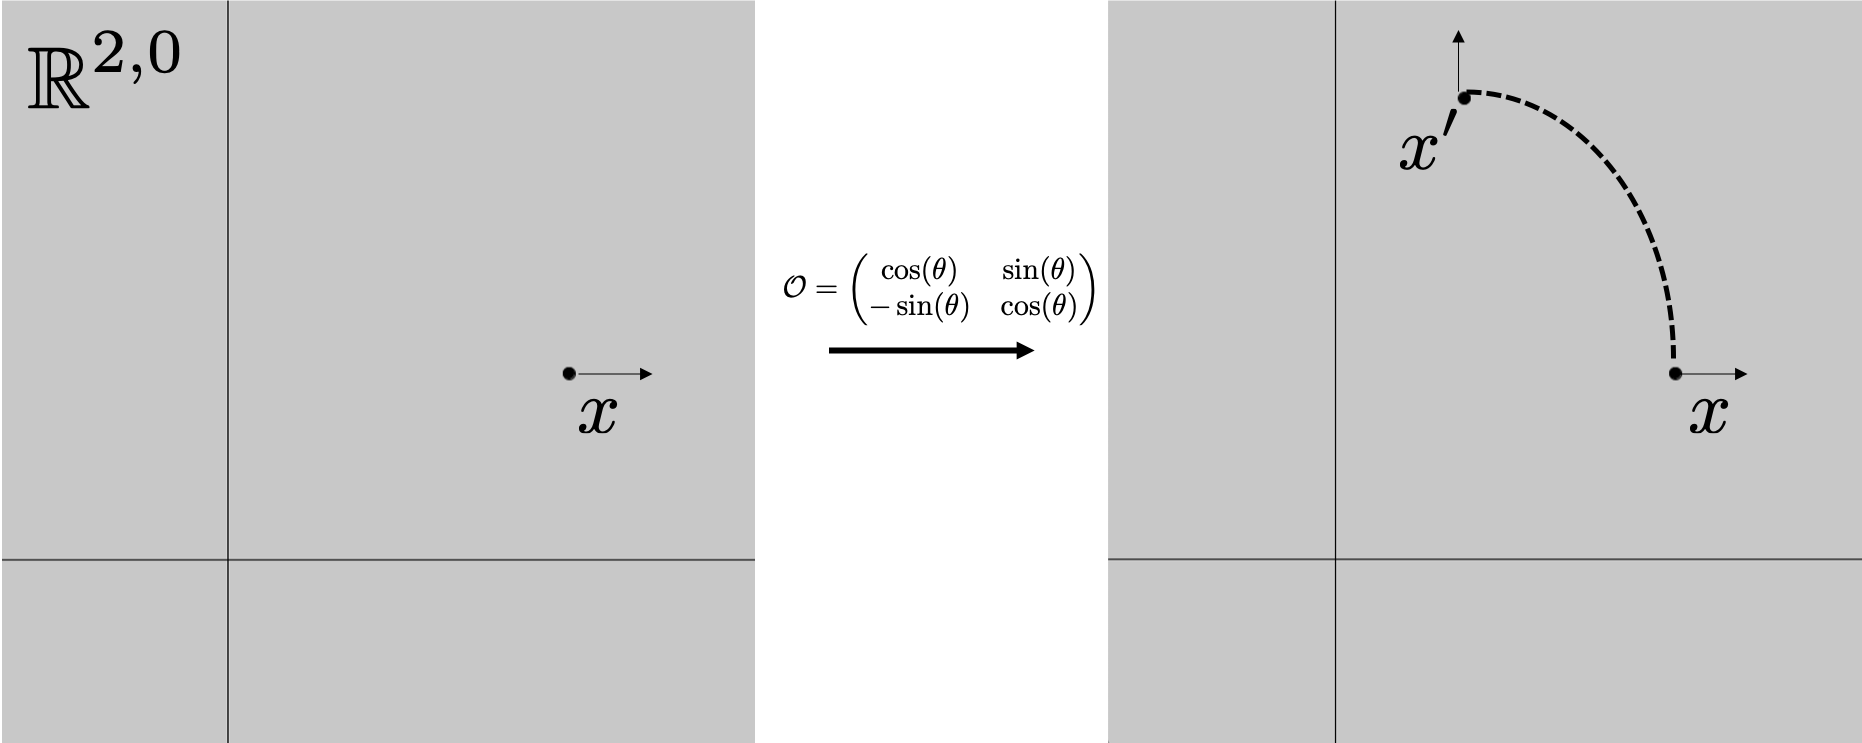
\includegraphics[width=4in]{images/active_rotation.png} 
\end{figure} 

\noindent After the rotation, the new field configuration at $x$ is

\begin{equation}
\phi'_a (x) = \sum_b \pi (\mathcal{O})_{ab} \phi_b (\mathcal{O}^{-1} x).
\end{equation}

\noindent The trivial representation of the field component $b$ would simply be the identity $\pi(\mathcal{O})_{ab} = \delta_{ab}$, and the fundamental, nontrivial representation is written

\begin{equation}
\pi (\mathcal{O})_{ab} = [ \mathcal{O} ] _{ab}.
\end{equation}

\noindent How does the action $S$ transform under a symmetry transformation?

\begin{equation}
S' = \int d^d x \, \Big{|} \text{det} \left( \frac{\partial x'^\mu}{\partial x^\nu} \right) \Big{|} \mathcal{L} \left( \mathcal{F} \left( \phi (x) \right), \frac{\partial x^\nu}{\partial x'^{\mu}} \partial_\nu \mathcal{F} \left( \phi (x) \right) \right)
\end{equation}

\noindent We also know that our theory is a conformal field theory, conformally invariant, conformally symemtric if the equations of motion are invariant. This is equivalent to the Lagrangian density transforming up to a total derivative

\begin{equation}
\mathcal{L}' = \mathcal{L} + \text{total derivative}.
\end{equation}

\noindent Now, let's study the infinitesimal generators of the conformal group $\text{Conf} ( \mathbb{R}^{p,q} )$.

\begin{itemize}
\item Translation
	\subitem $P_\mu = -i \partial_\mu$
\item Dilation
	\subitem $D = -i x^\mu \partial_\mu$
\item Rotation (Boost)
	\subitem $L_{\mu\nu} = i (x_\mu \partial_\nu - x_\nu \partial_\mu)$
\item Special Conformal
	\subitem $K_\mu = -i (2 x_\mu x'^\nu \partial_\nu - x^2 \partial_\mu)$
\end{itemize}

\noindent Work out the commutation relations to form a Lie algebra (\textbf{Exercise}).

\begin{align}
[D, P_\mu] &= i P_\mu \\
[D, K_\mu] &= -i K_\mu \\
[K_\mu, P_\nu] &= 2i (\eta_{\mu\nu} D - L_{\mu\nu} ) \\
[K_\rho, L_{\mu\nu}] &= i (\eta_{\rho\mu} K_\nu - \eta_{\rho\nu} K_\mu) \\
[P_\rho, L_{\mu\nu}] &= i (\eta_{\rho\mu} P_\nu - \eta_{\rho\nu} P_\mu ) \\
[L_{\mu\nu}, L_{\rho\sigma}] &= i (\eta_{\nu\rho} L_{\mu\sigma} + \eta_{\mu\sigma} L_{\nu\rho} - \eta_{\mu\rho} L_{\nu\sigma} - \eta_{\nu\sigma} L_{\mu\rho} )
\end{align}

\noindent And the rest commute. \\

\noindent Our task now is to find out which kinds of fields transform under the conformal group and give representations of the conformal group. We already know that a field transforming under $\text{Conf}(\mathbb{R}^{p,q})$, a general conformal transformation, transforms under the subgroup Poincar\'e, which is generated by translation $P_\mu$ and rotation $L_{\mu\nu}$, as

\begin{equation}
\phi_a (x) \rightarrow_{\text{Poincar\'e}} \sum_b \pi(\Lambda)_{ab} \phi_b (\Lambda^{-1}x).
\end{equation}

\noindent Let's focus on the subgroup of $\text{Conf}(\mathbb{R}^{p,q})$ which leave the orgin fixed: rotations, dilations, and SCTs. The infinitesimal generators of this subgroup form a subalgebra by exponentiation

\begin{equation}
\Lambda = e^{i \omega^\alpha G_\alpha}, \,\, \text{where } \omega^\alpha \text{ is infinitesimal.}
\end{equation}

\noindent The group element $G_\alpha$ can be $K_\mu$, $D$, or $L_{\mu\nu}$. At the origin, the Poincar\'e transformation  of the field looks like

\begin{equation}
\phi_a (x=0) \rightarrow \sum_b \pi (e^{i \omega^\alpha G_\alpha})_{ab} \phi_b (\Lambda^{-1} x = 0)
\end{equation}

\noindent Where the representation is, by Taylor expansion,

\begin{equation}
\pi(e^{i \omega^\alpha G_\alpha}) = \pi(\mathbb{I}) + i \omega^\alpha \pi(G_\alpha).
\end{equation}

\noindent Rename the representations of the generators (group elements)

\begin{align}
\pi(D) &= \tilde{\Delta} (\text{scaling dimension})\\
\pi(K_\mu) &= \kappa_\mu \\
\pi(L_{\mu\nu}) &= S_{\mu\nu} \, (\text{spin}).
\end{align}

\noindent The commutation of these representations are then

\begin{align}
[ \tilde{\Delta}, S_{\mu\nu} ] &= 0 \\
[ \tilde{\Delta}, \kappa_\mu ] &= -i \kappa_\mu \\
[ \kappa_\mu, \kappa_\nu ] &= 0.
\end{align}

\noindent Now, suppose that the generators $S_{\mu\nu}$ are irreducible representations, irreps, of the Lorentz group, the group that describes spin/helicity. By Schur's lemma (\textbf{Exercise}), we find that the scaling dimension is trivial, and, in turn, by the commuation relations, that all generators $\kappa_\mu$ are also trivial

\begin{equation}
\tilde{\Delta} \propto \mathbb{I} \implies -i \kappa_\mu = 0.
\end{equation}

\noindent Now use this fact to show how dilations act on the fields. The coordinates transform as

\begin{align}
x &\rightarrow \lambda x \\
x &\rightarrow \lambda^\epsilon \lambda^\epsilon \dots \lambda^\epsilon x
\end{align}

\noindent At the origin, the field transforms as

\begin{align}
\phi_a (x=0) \rightarrow&  (\mathbb{I} + i \epsilon \tilde{\Delta}) \dots (\mathbb{I} + i \epsilon \tilde{\Delta}) \phi_a (0) \\
&= \lambda^{i \tilde{\Delta}_a} \phi_a (0) \\
&= \lambda^{-\Delta_a} \phi_a (0)
\end{align}


\noindent Where we used the Taylor expansion of the infinitesimal $\epsilon$, and the last line uses $\tilde{\Delta} = i \Delta \mathbb{I}$, since Schur's lemma tells us that the scaling deimension is trivial. \\

\noindent So, every conformal field has a behavior under dilations, defined by the scaling dimension $\Delta_a$, with Jacobian

\begin{equation}
\Big{|} \frac{\partial x'}{\partial x} \Big{|} = \Lambda^{-\frac{d}{2}}, \text{ where } \Lambda = \lambda^{-2}.
\end{equation}

\noindent And the metric transforms under dilations as

\begin{equation}
g'_{\mu\nu} = \lambda^{-2} g_{\mu\nu}.
\end{equation}

\noindent Putting all this together, the field now transforms as 

\begin{equation}
\phi_a (x) \rightarrow \phi'_a (x') = \Big{|} \frac{\partial x'}{\partial x} \Big{|}^{-\frac{\Delta}{d}} \phi_a (x).
\end{equation}

\noindent Filling in the Jacobian, the new field in terms of the orignial field and the original spacetime location is

\begin{align}
\phi'_a (x) &= \sum_b \pi(\Lambda)_{ab} \phi_b (\Lambda^{-1} x) \\
&= \sum_b [ \lambda^{-\Delta}]_{ab} \phi_b (\Lambda^{-1} x) \\
&= \lambda^{-\Delta} \phi_a (\Lambda^{-1} x) \\
&= \lambda^{-\Delta} \phi_a (\lambda^{-1} x).
\end{align}

\noindent By the Baker-Campbell-Hausdorff (BCH) formula, we know how the new field looks at all spacetime lcoations, not just the origin (\textbf{Exercise})

\begin{align}
e^{i x^\rho P_\rho} D e^{-i x^\rho P_\rho} &= D + x^\nu P_\nu \\
&\implies D \phi_a (x) = (-i x^\nu \partial_\nu + \tilde{\Delta} ) \phi_a (x).
\end{align}

\noindent In the next lecture, we give this the quantum treatment, where we will look for unitary representations (self-adjoint operators), that are labelled by quantum numbers, such as spin, scaling dimension, and central charge. The central charge will require projective unitary representations.
